%

%%%%%%%%%%%%%%%%%%%%%%%%%%%%%%%%%%%%%%%%%%%%%%%%%%%%%%%%%%%%%%%%%%%%%%%%
\chapter{Plugin}
\label{chap:Plugin}

In this chapter, I will explain what the plugin has to offer, how the user interface is designed and how it internally works. I will also give insight into my reasoning during development about why I chose to implement things as I did. This includes outlining alternative solutions which I have taken into consideration but eventually abandoned.

%%%%%%%%%%%%%%%%%%%%%%%%%%%%%%%%%%%%%%%%%%%%%%%%%%%%%%%%%%%%%%%%%%%%%%%%
\section{Goals}
\label{sec:goals}

The main goal of this plugin was to teach students how messages are encrypted using the ChaCha cipher family. It should focus on creating an easy to understand visualization of its internals without oversimplification.
It should further visualize the diffusion property of the cipher on demand by making it possible for the user to enter secondary values for the key, initialization vector and initial counter.

The plugin should support all variants of the cipher. This means that the user should be able to choose the key size (128-bit or 256-bit) and how often the hash function should be executed per keystream block (8, 12 or 20 rounds). 
Since the Internet Engineering Task Force (IETF) introduced a slightly modified version of ChaCha which uses a 32-bit counter and 96-bit initialization vector, the user can also decide if the wants to use the original version by Daniel J. Bernstein with a 64-bit counter and 64-bit initialization vector or the one described by the IETF.

%%%%%%%%%%%%%%%%%%%%%%%%%%%%%%%%%%%%%%%%%%%%%%%%%%%%%%%%%%%%%%%%%%%%%%%%
\section{Implementation details}
\label{sec:implementationDetails}

\blindtext[1]

%%%%%%%%%%%%%%%%%%%%%%%%%%%%%%%%%%%%%%%%%%%%%%%%%%%%%%%%%%%%%%%%%%%%%%%%

\subsection{Key Features}
\label{sec:keyFeatures}

\blindtext[2]

\subsection{User Interface}
\label{sec:userInterface}

\blindtext[8]

\subsection{Architecture}
\label{sec:Architecture}

\blindtext[8]

%%%%%%%%%%%%%%%%%%%%%%%%%%%%%%%%%%%%%%%%%%%%%%%%%%%%%%%%%%%%%%%%%%%%%%%%

\section{Encountered Problems}
\label{sec:encounteredProblems}

In this section, I will discuss the main problems I encountered during implementation. To briefly summarize, they mainly consisted of how to create a simple, intuitive user interface and how the system behind the interface should be designed to have the best or at least a reasonable performance. \\ In the other visualizations, I noticed that I was quite overwhelmed by the amount of buttons which were visible, even though not always enabled. So I wanted to keep my user interface as simple as possible while not restricting the user in his ability to navigate through the visualization. \\ Regarding the performance, the author of the AES visualization has mentioned in his thesis that to create a fluent user experience where he can navigate back and forth between all steps, the intermediate values need to be calculated beforehand and saved since we don't want to stop at each step to calculate the next value or recalculate everything from the start if the user wants to go backwards. I came to the same conclusion. But as I will describe on the next pages, this was not all that was needed to ensure such an experience.\\
I hope that the description of these problems and the solutions I have found may help future students in writing their own plugins.

\subsection{Performance}

\subsubsection{Linear navigation system}

The peformance of the plugin was essentially coupled to how the navigation system was designed. Other things like the aforementioned calculation of the intermediate values for the visualization were compared to the navigation system design unsignificant because they are created by the ChaCha cipher anyway and must just be saved somewhere to not lose them. This means that storing them was only a necessary but not sufficient condition for a overall good performance. I realized this early in development when I had my first page with many page actions on it and wanted to skip ahead a lot of actions. While implementing this feature which would enable the user to skip from any action to any other action, I realized that when skipping more than 100 actions, it already took about 750ms during which the UI was unresponsive. As can be seen in \ref{navsystem.linear.stats}, this time increased linearly so it was quite clear that I needed to do something about this, especially because the page with the most actions had over 3000 single actions.

\par

The root cause of the problem was the navigation system design which I called in hindsight \textbf{\textit{linear navigation system}}. It consisted of defining actions which build upon each other. This means that if we are at action 0 (initial state of the page) and want to go to action 5, we need to execute all the code inside the action definitions between 0 and 5 to arrive at the page state as it should be at action 5. This is resembled in Figure \ref{navsystem.linear.overview}.

\begin{figure}
\caption{Navigation paths between actions in the linear navigation system}
\label{navsystem.linear.overview}
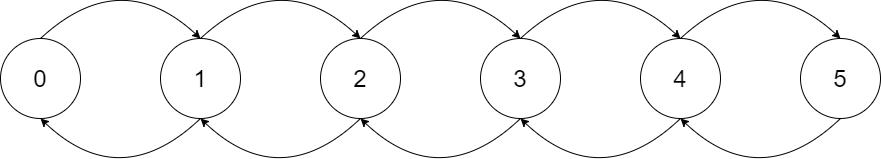
\includegraphics[width=\textwidth]{figures/navigationsystem-linear-overview.png}
\end{figure}

I came up with this design to have a smooth implementation experience where I only have to write the actual page state changes between two actions instead of duplicating a lot of code since the page state changes which were applied during a previous page were most of the times still visible when moving to the next action. This complements how the user experiences the visualization because the actions are numbered in a sequence and thus are inherently linear. Because of this, it made a lot of sense to me to reflect this in the system architecture.

\par

Since this "design flaw" was not the leading cause of the performance problem (going through a for-loop of size 3000 does not directly lead to performance issues), I want to briefly explain how the actual action implementation looked like.\\
As can be seen in Figure \ref{navsystem.linear.detail}, during the transition between two page states, the state of the page elements which will change is saved such that we can undo the changes if the user decides to navigate back. This enabled me to skip writing action definitions for backwards navigation, since I could just write a function which retrieves the state corresponding to the transition and then applies it. This function would then work for all backwards navigation without further intervention which was very convenient during development.
The problem with that architecture was that the state saving and the execution logic inside the action definitions were changing a lot of page elements directly by accessing them via their name that I gave them in the XAML code. That this was against best practices in writing WPF applications I only noticed later on, when I read more about them. This issue combined with the restricted, linear pathing between actions resulted in that huge performance loss that was described in Figure \ref{navsystem.linear.stats}.

\subsubsection{Linear navigation system with caches}

After identifying the two underlying issues, I implemented what I called a \textbf{\textit{linear navigation system with caches}}. As the name suggests, I implemented cache entries to be able to navigate in constant time between an action and an action for which I created a cache. To not only increase peformance during these transitions but between all transitions, we check before each transition, if first moving to a cached entry would decrease the amount of hops needed to go to our destination.

\par

The cache entries consisted of instructions to restore the complete state of a page at the action index for which this cache entry was for. They contained instructions for the complete state instead of only the difference between two actions because now, moving to that cache must initialize the page, independent at which action / page state we were before. This means that there was some overhead in initializing the page because essentially, I cleared the whole page and then initialized the page elements with their appropriate content, potentially leading to some unnecessary code execution because the content prior to cleaning was already the one we needed. But this overhead was . Figure \ref{navsystem.cache.overview} demonstrates that the navigation system now needs less hops between any two given actions. This increased performance significantly as can be seen in \ref{navsystem.cache.stats}. \par

\begin{figure}
\caption{Navigation paths between actions in the linear navigation system with caches. The colorized state has a corresponding cache entry.}
\label{navsystem.cache.overview}
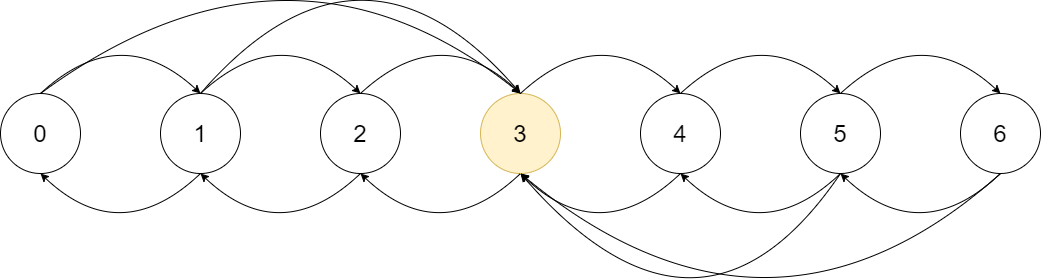
\includegraphics[width=\textwidth]{figures/navigationsystem-cache-overview-2.png}
\end{figure}

Further, to decrease the load on the CPU while dragging the action slider, I implemented a very simple asynchronous navigation. It was implemented by using a stack as a buffer for the values received from the values during dragging. Every 50ms, the last value from the buffer is read and the page moves to that action. Afterwards, the buffer is cleared. This did only enhance the slider but not the overall performance because at its core, it used the same navigation logic; just asynchronously. Nonetheless, it improved the performance during dragging significantly which I found quite impressing for how minimal the code for it is. In fact, the whole code for the asynchronous navigation can be seen in Figure \ref{async.navigation}.

\begin{figure}
\caption{Asynchronous navigation subsystem}
\label{async.navigation}
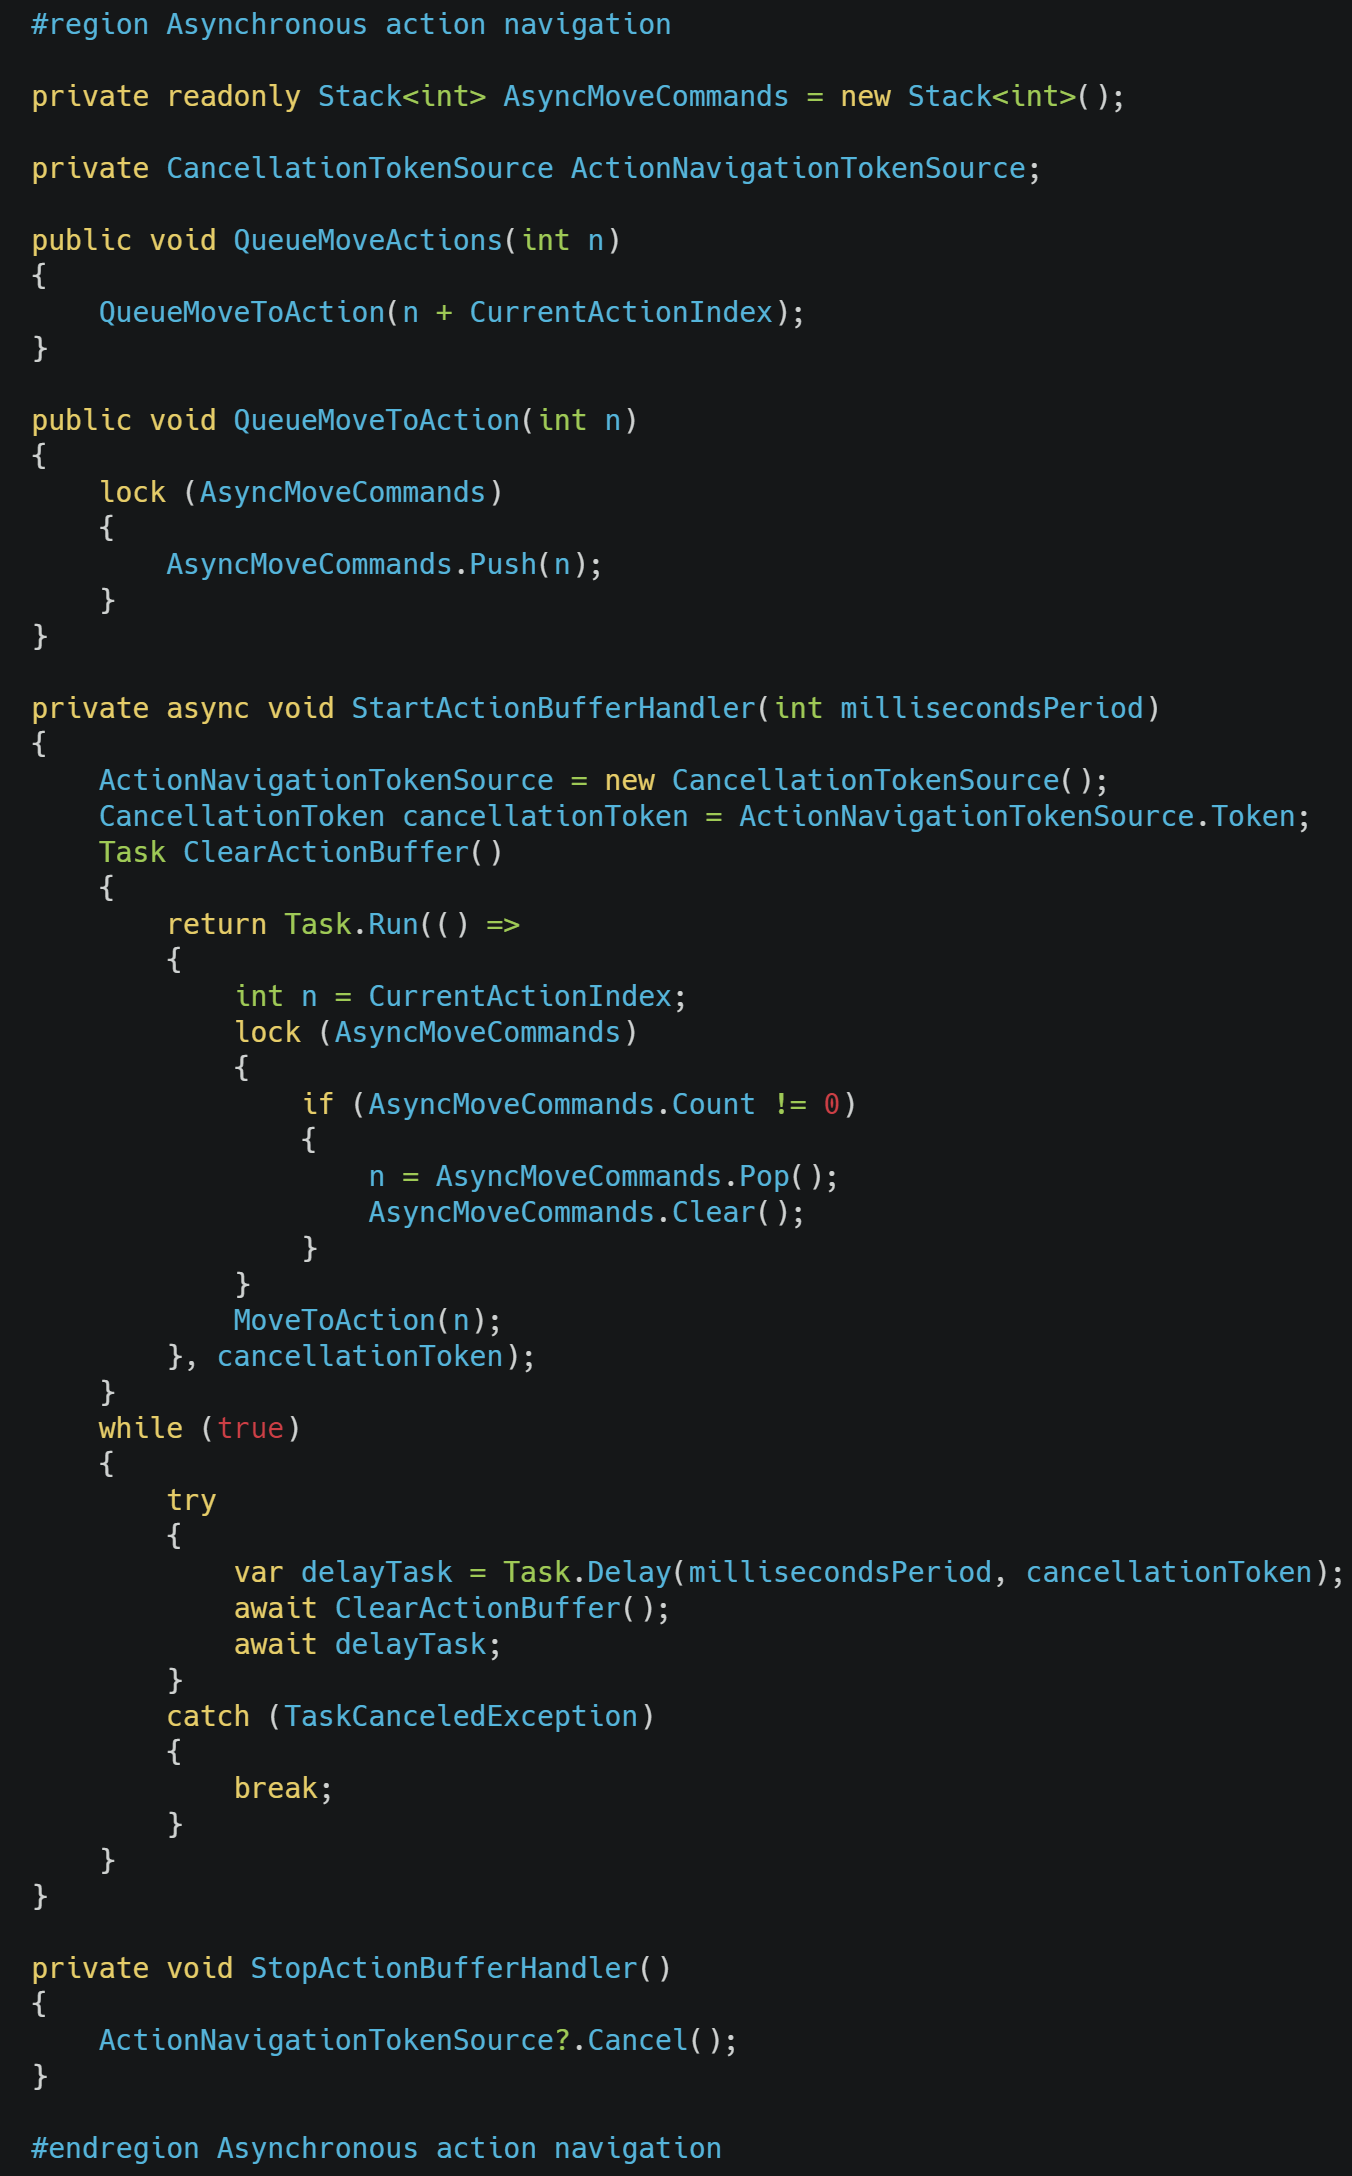
\includegraphics[width=\textwidth]{figures/async-navigation.png}
\end{figure}

One of the major drawbacks for this enhanced design was that the automatic action undoing was no longer possible. Since we can not guarantee that the state between two actions has been saved, we cannot use our undo function. The reason is that any transition between two actions may have been skipped because first moving to a cached entry needed less hops. Therefore, I needed to write the code for backwards navigation to support caching.

\subsubsection{Centralized navigation system}

While implementing other features such as the diffusion, I noticed that having to implement for each page action the forward and backwards code, my code became quite error-prone. It was hard to notice bugs because it was not feasible to check every single action from both directions manually and creating a testing framework just because of this was out of scope. Some navigation bugs were easy to find because due to the overall still linear nature of the navigation system, errors did propagate. This means that a error in a previous action most likely did break the page state on future actions because they depend on each other. Nonetheless, this did not help in tracking down the bug because I did not know on which action the error happened. This only further incentivised me to reiterate on the navigation system again.

\par

I summarized all the problems I currently had with my code which not only consisted of performance problems but also with visualization problems such as scaling or being quite restricted in what the current navigation system supported. Since I only updated the existing code during the last time I revisited the navigation system, the core design was still all about directly manipulating and creating UI elements on demand. I did use a lot of code-behind which was highly coupled to the XAML code because it was very straight-forward to do so and lead to fast results. At first, I thought the trade-off between loss of maintainability/flexibility in the future and not having to spend precious time to learn design patterns for WPF applications was worth it. I thought so because I was not writing an enterprise application on which the long-term success of a company depended and which would get regular updates in the future thus high maintainability or being easy to extend was not a priority

\par

I got proven wrong when I realized I already reached the limit of "code smells" which slowed me down in updating, fixing or creating new features. What follows is the list of problems together with what requirement the new navigation system needs to meet to solve them:

\begin{description}
\item [(Inconsistent) Performance] The underlying linear design was crippling the performance for the reasons already mentioned. The introduction of caches did only fight the symptoms but did not solve the main issue. Further, it made the performance confusing for the users since sometimes, it took close to no time at all to move to a certain action but on the other hand, it sometimes took quite a lot of time to move to a different action (because it was not cached). \\
\textit{\textbf{Requirement}}: Moving to any action should be done in $O(1)$. This means, it should not matter how many actions we needed to skip to arrive at the destination.
\item [Error-prone design for action creation] Writing new actions was error-prone because I needed to write code for forward and backwards navigation which introduced mental overhead because it depended on the code of all previous actions. This also lead to error propagation. Errors were easily noticeable by users but were hard to track down to their origin ("snowball effect").\\
\textit{\textbf{Requirement}}: New actions should be able to be written without having to write backwards navigation code. Backwards navigation should be handled automatically and thus be "error-free by design".
\item [No coherent system design] Adding new code without following a design pattern made it hard to grasp the system architecture over the long run. Additionally, the high coupling of the backend (code-behind) with the frontend (XAML) made it harder to implement new features in one part without needing to modify the other part. The system essentially got very rigid and over time, even conceptual small changes needed a lot of effort to implement.\\
\textit{\textbf{Requirement}}: The new system should make it clear what piece of code is responsible for what and thus be highly modular. This should also make it clear where new code must be added to implement a new feature without increasing technical debt.
\end{description}

\subsubsection{Centralized navigation system}
